%pdflatex --shell-escape scap_benchmark_dl_training
%biber scap_benchmark_dl_training 

\PassOptionsToPackage{hyphens}{url}
\documentclass[compress,aspectratio=169]{beamer}

\usepackage[official]{eurosym}
\usepackage{multirow}
\setlength{\marginparwidth}{2cm}
\usepackage{todonotes}
\presetkeys{todonotes}{inline}{}
\usepackage[style=verbose,backend=biber,style=authoryear, citestyle=authoryear ]{biblatex}
\setbeamertemplate{bibliography item}{\insertbiblabel} % Ensure that cite labels appear in references section
\addbibresource{ref.bib}
\usepackage{./assets/beamerthemeGoettingen} % make sure the theme file is on this path
\graphicspath{{../}{./assets/}}
\usepackage{caption}
\usepackage{booktabs}

\hypersetup{
    colorlinks,
    citecolor=black,
}

\newcommand{\source}[1]{\par\begin{textblock*}{6cm}(1cm,8cm)
    \begin{beamercolorbox}[wd=\paperwidth,ht=0.5cm,right]{framesource}
        \usebeamerfont{framesource}\usebeamercolor[fg]{framesource} \centering\tiny {#1}
    \end{beamercolorbox}
\end{textblock*}}


% listing / code
\usepackage{minted}
\usemintedstyle{tango}
% Box listing / code
\usepackage{tcolorbox}

% Box listing / code style 
% These options will be applied to all `tcolorboxes`
\tcbset{%
    noparskip,
    colback=gray!5, %background color of the box
    colframe=gray!20, %color of frame and title background
    coltext=black, %color of body text
    coltitle=black, %color of title text 
    fonttitle=\tiny,
    alerted/.style={coltitle=red, 
                     colframe=gray!40},
    example/.style={coltitle=black, 
                     colframe=green!20,             
                     colback=green!5},
    }

\lstset{literate=%
    {Ö}{{\"O}}1
    {Ä}{{\"A}}1
    {Ü}{{\"U}}1
    {ß}{{\ss}}1
    {ü}{{\"u}}1
    {ä}{{\"a}}1
    {ö}{{\"o}}1
    {~}{{\textasciitilde}}1
}

\usepackage{csquotes} % For \enqoute{}
\usepackage{hyperref}

% --- document configuration ---
\newcommand{\mytitle}{Getting started with profiling PyTorch}     
% Leave empty for no subtitle
\newcommand{\mysubtitle}{State of the art and plan for Scalable Computing Systems and Applications in AI, Big Data and HPC}   
\newcommand{\myauthor}{Hauke Kirchner}
\newcommand{\myauthorurl}{\href{http://www.overleaf.com}{Something 
Linky}}
\newcommand{\myvenue}{Göttingen}
% For example, use \today
\newcommand{\mydate}{24.11.2022}
% For example, Institute for Computer Science / GWDG
\newcommand{\myinstitute}{GWDG - AG Computing}
% Leave empty for no footer image
\newcommand{\myfooterimage}{}           
\newcommand{\mygrouplogo}{}
% Images must be enabled manually under title page \titleLogo
% Adjust position and width manually for fewer images
\newcommand{\mytitleimageone}{}         
\newcommand{\mytitleimagetwo}{}        
\newcommand{\mytitleimagethree}{}

% --- title page ---
\title{\Large \mytitle}
\venue{\myvenue}
\date{\mydate}
\subtitle{\mysubtitle}
%\authorURL{\myauthorurl}
\author{{\myauthor}}
\authorFooter{\myauthor \hspace{0.3cm} \includegraphics[height=1em]{\myfooterimage}}
\institute{\myinstitute}
%\groupLogo{\includegraphics[width=2cm]{\mygrouplogo}}
\titleLogo{
%\includegraphics[height=2.7cm]{\mytitleimageone}
%\includegraphics[height=2.7cm]{\mytitleimagetwo}
%\includegraphics[height=2.7cm]{\mytitleimagethree}
}

\setbeamertemplate{footline}[text line]{
\begin{beamercolorbox}[sep=0.5em,wd=\paperwidth,leftskip=0.2cm,rightskip=0.1cm]{footlinecolor}
\myauthor \hfill \insertVenue \hfill \insertframenumber\,/\,\ref{pg:lastpage}
\end{beamercolorbox}
}

\begin{document}

\begin{frame}[plain]
	\titlepage
\end{frame}

\begin{frame}{Course Agenda}
\centering
\includegraphics[width=0.9\textwidth]{assets/dlgpu_agenda}
\end{frame}

\begin{frame}[t]{Table of contents}
  \tableofcontents[subsectionstyle=hide/hide]
\end{frame}

% --- slides begin ---

\section{Motivation}

\begin{frame}{Why is it important to profile the training process of neural networks?}

    \begin{columns}
        \begin{column}{0.5\textwidth}
            \begin{block}{\centering Training speed}
                \centering
                \vspace{3em}
                
\includegraphics[width=0.3\textwidth]{assets/speed_FILL0_wght400_GRAD0_opsz48.png}
            \end{block}
        \end{column}
        \begin{column}{0.5\textwidth}
            \begin{block}{\centering Energy efficiency}
                \centering
                \vspace{3em}
                
\includegraphics[width=0.3\textwidth]{assets/electric_bolt_FILL0_wght400_GRAD0_opsz48}
            \end{block}
        \end{column}
    \end{columns}

\end{frame}

\begin{frame}{Training speed 
              \begin{tabular}{@{}c@{}}
                  
\includegraphics[width=0.05\textwidth]{assets/speed_FILL0_wght400_GRAD0_opsz48.png}
              \end{tabular}
              }

    \vspace{-3em}

    \begin{columns}
        \begin{column}{0.6\textwidth}
            \begin{itemize}
                \item training of neural networks is computationally intensive
                \item[$\hookrightarrow$] workflow needs to be optimized for available hardware
                    \begin{itemize}
                        \item How to make good use of clusters with heterogenous hardware?
                        \item How many GPUs are worth requesting?
                    \end{itemize}
                    \vspace{2em}
                \item[$\Rightarrow$] optimization for available accelerators is critical in ML/DL
            \end{itemize}
        \end{column}
        \begin{column}{0.4\textwidth}
            \vspace{-1em}
            \begin{figure}
                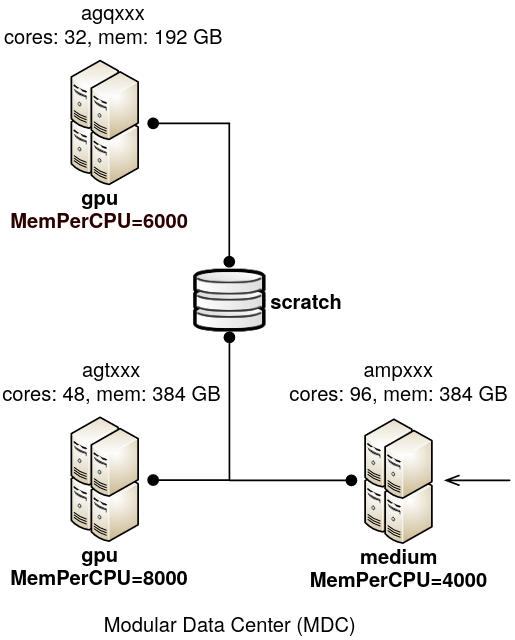
\includegraphics[width=0.9\textwidth]{assets/gwdg_scc.png}
                \caption*{Structure and resources of a part of the Scientific Compute Cluster.}
            \end{figure}
        \end{column}
    \end{columns}

    \source{Image source: Adapted from \url{https://www.gwdg.de/web/guest/hpc-on-campus/scc}, accessed on: 09.11.2022}
\end{frame}

\begin{frame}{Energy efficiency 
              \begin{tabular}{@{}c@{}}
                  
\includegraphics[width=0.05\textwidth]{assets/electric_bolt_FILL0_wght400_GRAD0_opsz48}
              \end{tabular}
              }



    \begin{columns}
        
        \begin{column}{0.6\textwidth}
            \begin{itemize}
                \item idea of \textbf{GreenAI}~(\cite{schwartz_2019_greenai})\\[1em]
                \item very different energy requirements (finetuning vs training)\\[1em]
                \item deep learning is emerging in several fields
                    \begin{itemize}
                        \item[$\Rightarrow$] the impact on energy consumption and consequently, our climate is growing
                    \end{itemize}
            \end{itemize}
        \end{column}

        \begin{column}{0.4\textwidth}
            \vspace{-3.5em}
            \centering
            \begin{figure}
            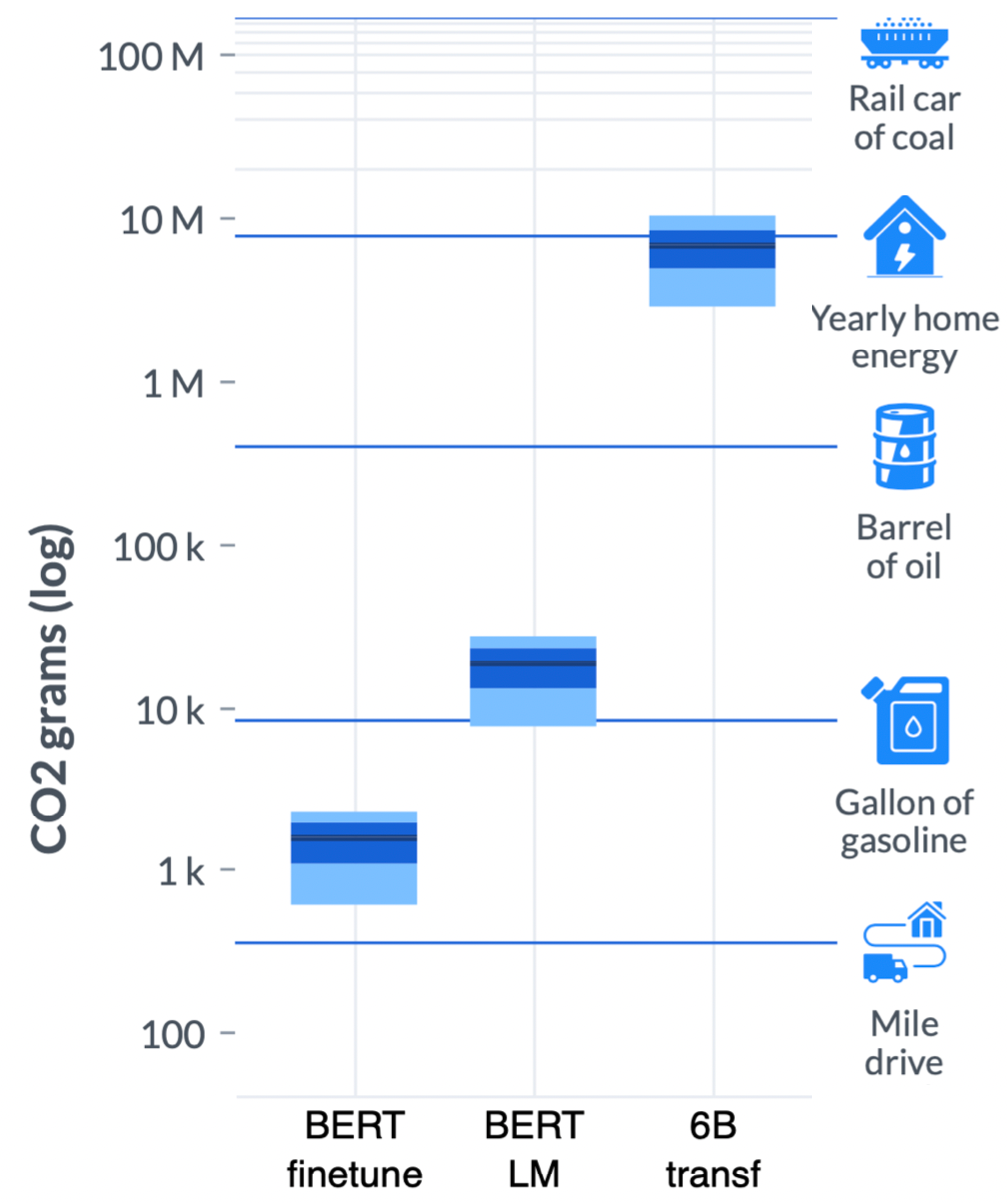
\includegraphics[width=\textwidth]{assets/20220610_dodge_measuring-the-carbon-intensity-of-ai-in-cloud-instances-fig2-bert.png}
            \caption*{$CO_2$ Relative Size Comparison}
            \end{figure}
            \source{Image source: Adapted from \cite{20220610_dodge_measuring-the-carbon-intensity-of-ai-in-cloud-instances}}
            
        \end{column}
    \end{columns}



\end{frame}

\section{Methods}
\sectionIntroHidden % Show an outline of the current section with hidden subsections
%\sectionIntro % Show an outline of the current section with subsections

\begin{frame}{Metrics}

% Please add the following required packages to your document preamble:
% \usepackage{booktabs}
% \usepackage{multirow}
\begin{table}[]
\begin{tabular}{@{}ll@{}}
\toprule
metric                                                                                 & purpose                        \\ \midrule
Execution time                                                                         & \multirow{2}{*}{traditionally} \\
FLOPS                                                                                  &                                \\ \midrule
Throughput: $\frac{images}{sec}$                                                       & with the advent of GPUs        \\ \midrule
Time to Accuracy (TTA)                                                                 & \multirow{2}{*}{deep learning} \\
\begin{tabular}[c]{@{}l@{}}Average Time to \\ Multiple Thresholds (ATTMT)\end{tabular} &                                \\ \bottomrule
\end{tabular}
\end{table}


\source{Image source: Adapted from \url{https://snehilverma41.github.io/Metrics_ML_FastPath19.pdf}}

\end{frame}


\section{Tool overview}
\sectionIntroHidden

\begin{frame}[t]{Tools}
    \begin{center}
        
\includegraphics[width=1\textwidth]{./assets/tools}
    \end{center}
    \begin{columns}[t]
    \begin{column}{0.5\textwidth}
                \begin{itemize}
                    \item PyTorch - Profiler~\footnote{\tiny{\url{https://pytorch.org/tutorials/intermediate/tensorboard_profiler_tutorial.html}}}
                    \item collection of performance metrics
                    \item indentification of\\expensive operators
                    \item tracking of the kernel activity
                \end{itemize}
    \end{column}
    \begin{column}{0.5\textwidth}
                \begin{itemize}
                    \item FlopsProfiler~\footnote{\tiny{\url{https://www.deepspeed.ai/tutorials/flops-profiler/}}}
                    \item model speed (latency, throughput)
                    \item efficiency (FLOPS\footnote{\tiny{floating-point operations per second}})
                \end{itemize}
    \end{column}
    \end{columns}
\end{frame}

\section{PyTorch Profiler}
\sectionIntroHidden

\begin{frame}{PyTorch Profiler With TensorBoard}
    \vspace{-1em}
    \begin{center}
    \begin{figure}
        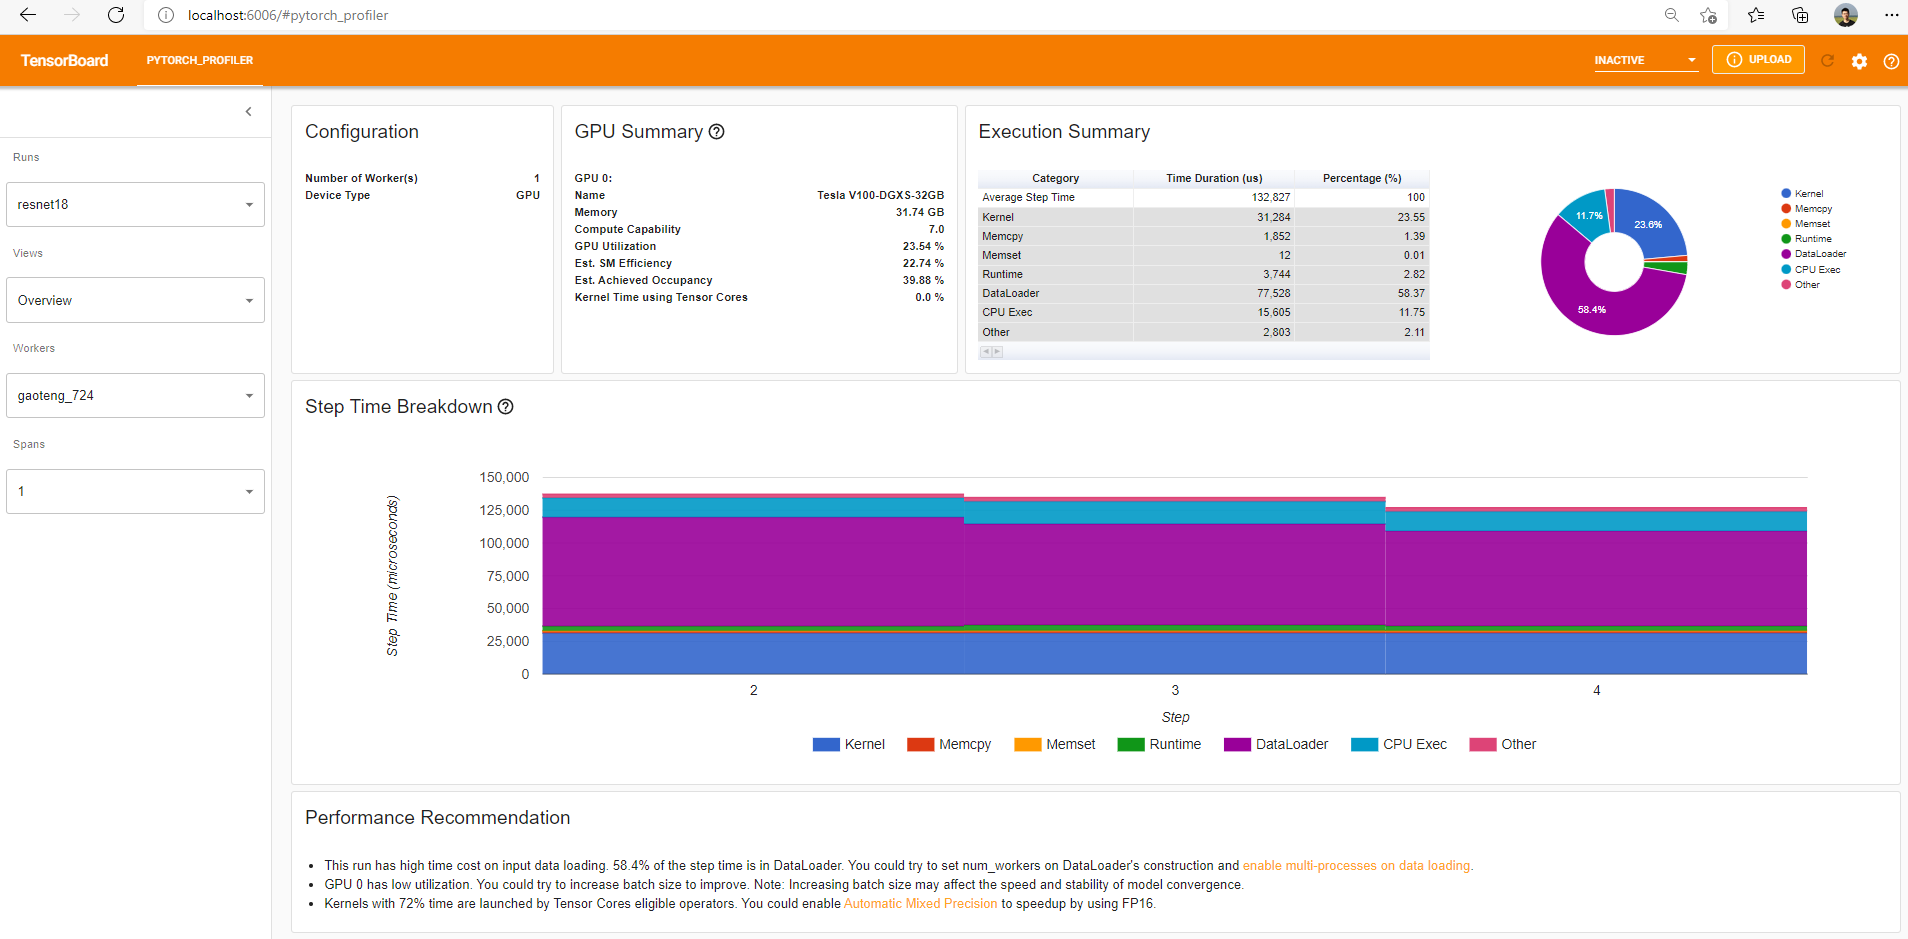
\includegraphics[width=1\textwidth]{assets/profiler_overview1}
    \end{figure}
    \end{center}
\source{Image source: \url{https://pytorch.org/tutorials/intermediate/tensorboard_profiler_tutorial.html}, accessed on: 22.11.2022}

\end{frame}

\begin{frame}{PyTorch Profiler With TensorBoard}
    \vspace{-1em}
    \begin{center}
    \begin{figure}
        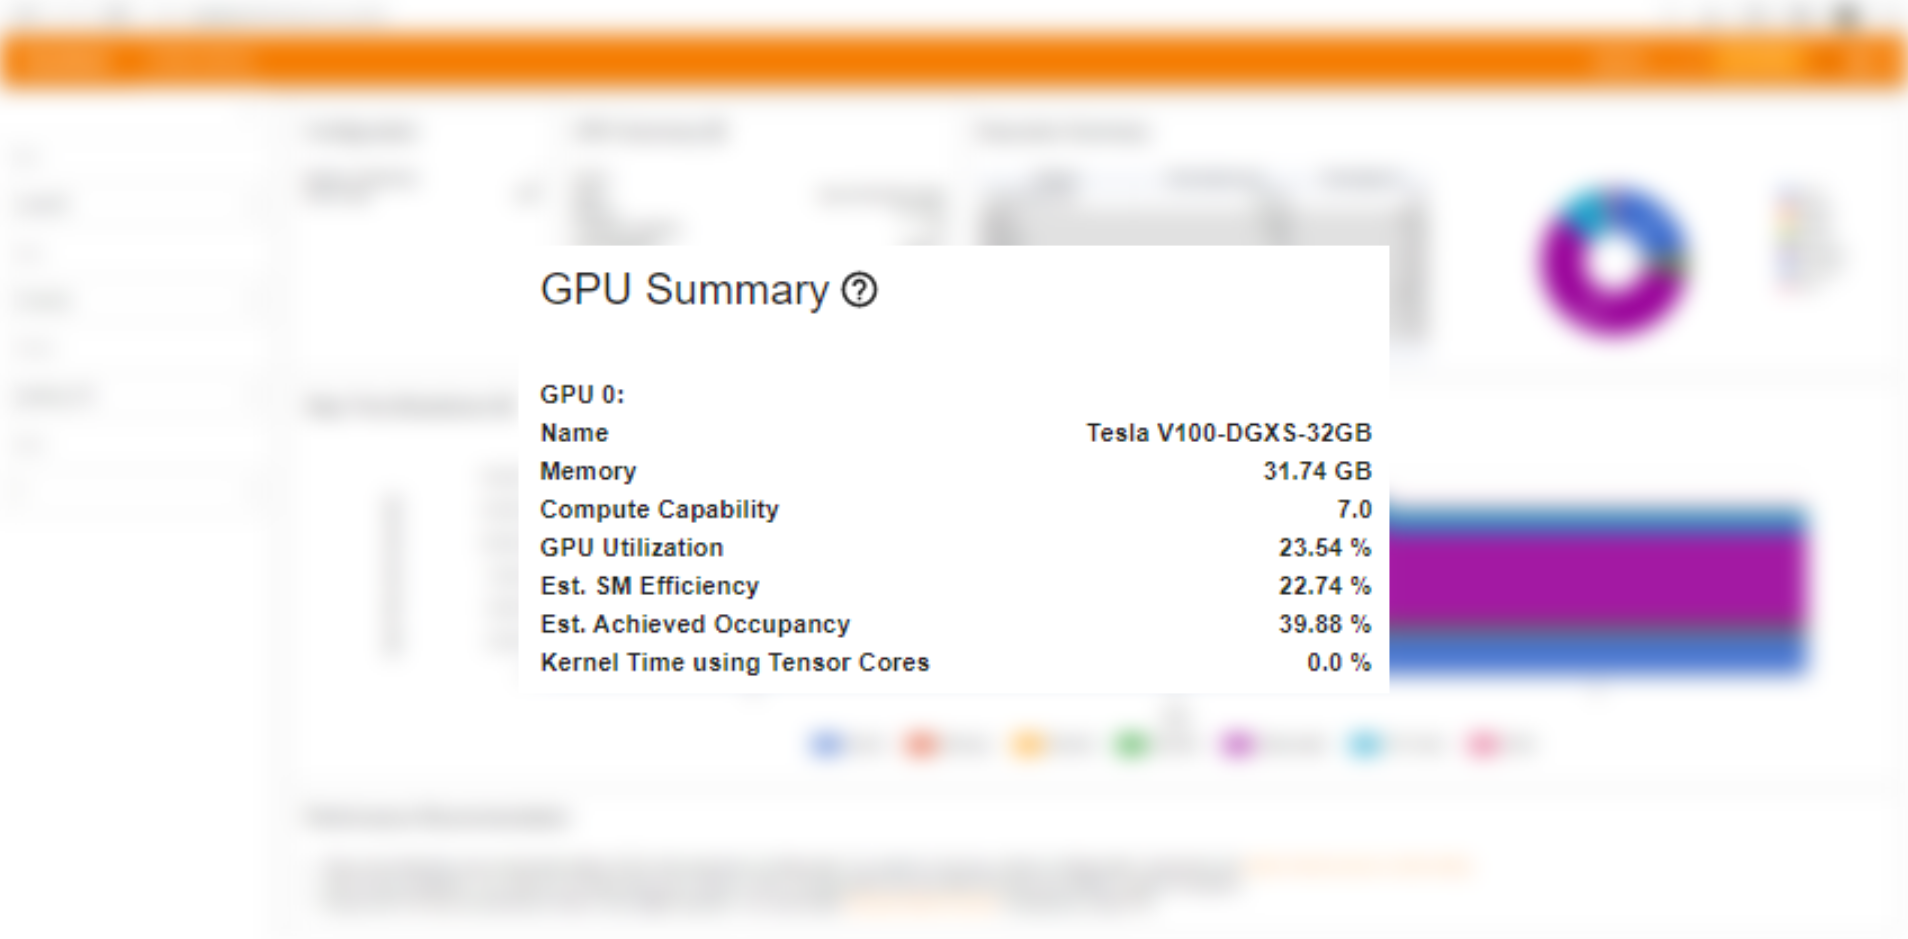
\includegraphics[width=1\textwidth]{assets/profiler_overview_gpu_summary}
    \end{figure}
    \end{center}
\source{Image source: Adapted from \url{https://pytorch.org/tutorials/intermediate/tensorboard_profiler_tutorial.html}, accessed on: 22.11.2022}

\end{frame}

\begin{frame}{PyTorch Profiler With TensorBoard}
    \vspace{-1em}
    \begin{center}
    \begin{figure}
        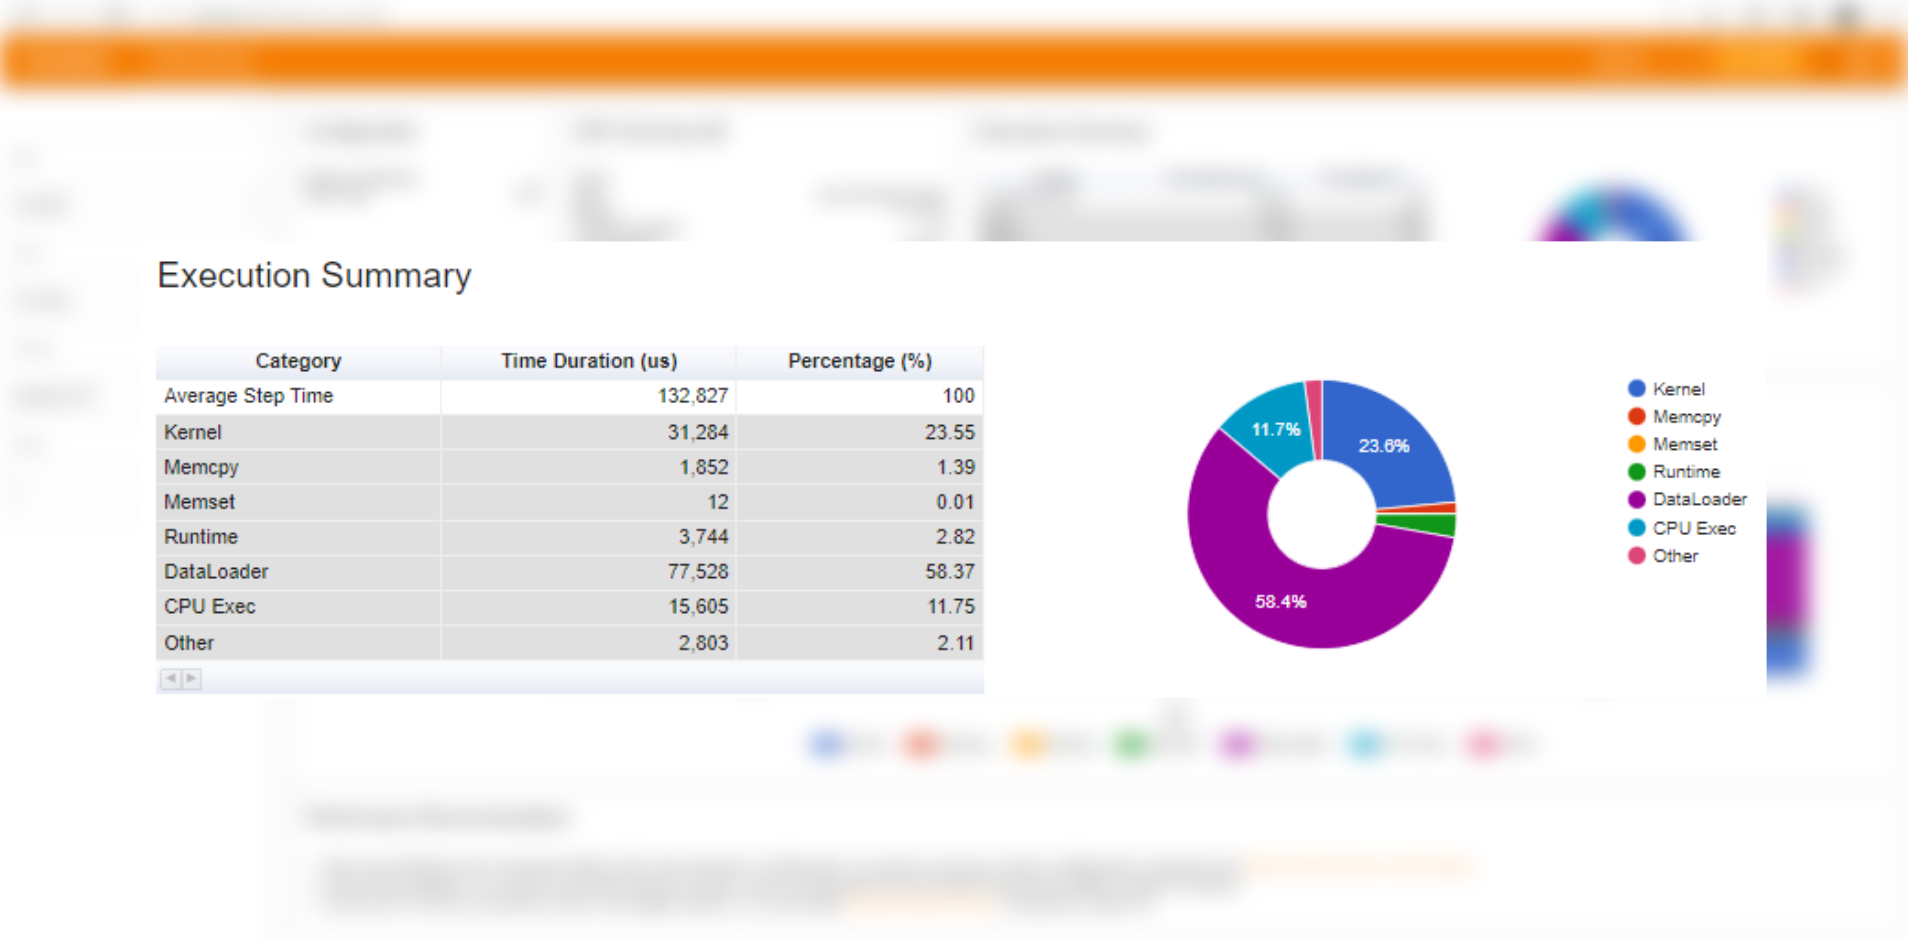
\includegraphics[width=1\textwidth]{assets/profiler_overview_execution_time}
    \end{figure}
    \end{center}
\source{Image source: Adapted from \url{https://pytorch.org/tutorials/intermediate/tensorboard_profiler_tutorial.html}, accessed on: 22.11.2022}

\end{frame}

\begin{frame}{PyTorch Profiler With TensorBoard}
    \vspace{-1em}
    \begin{center}
    \begin{figure}
        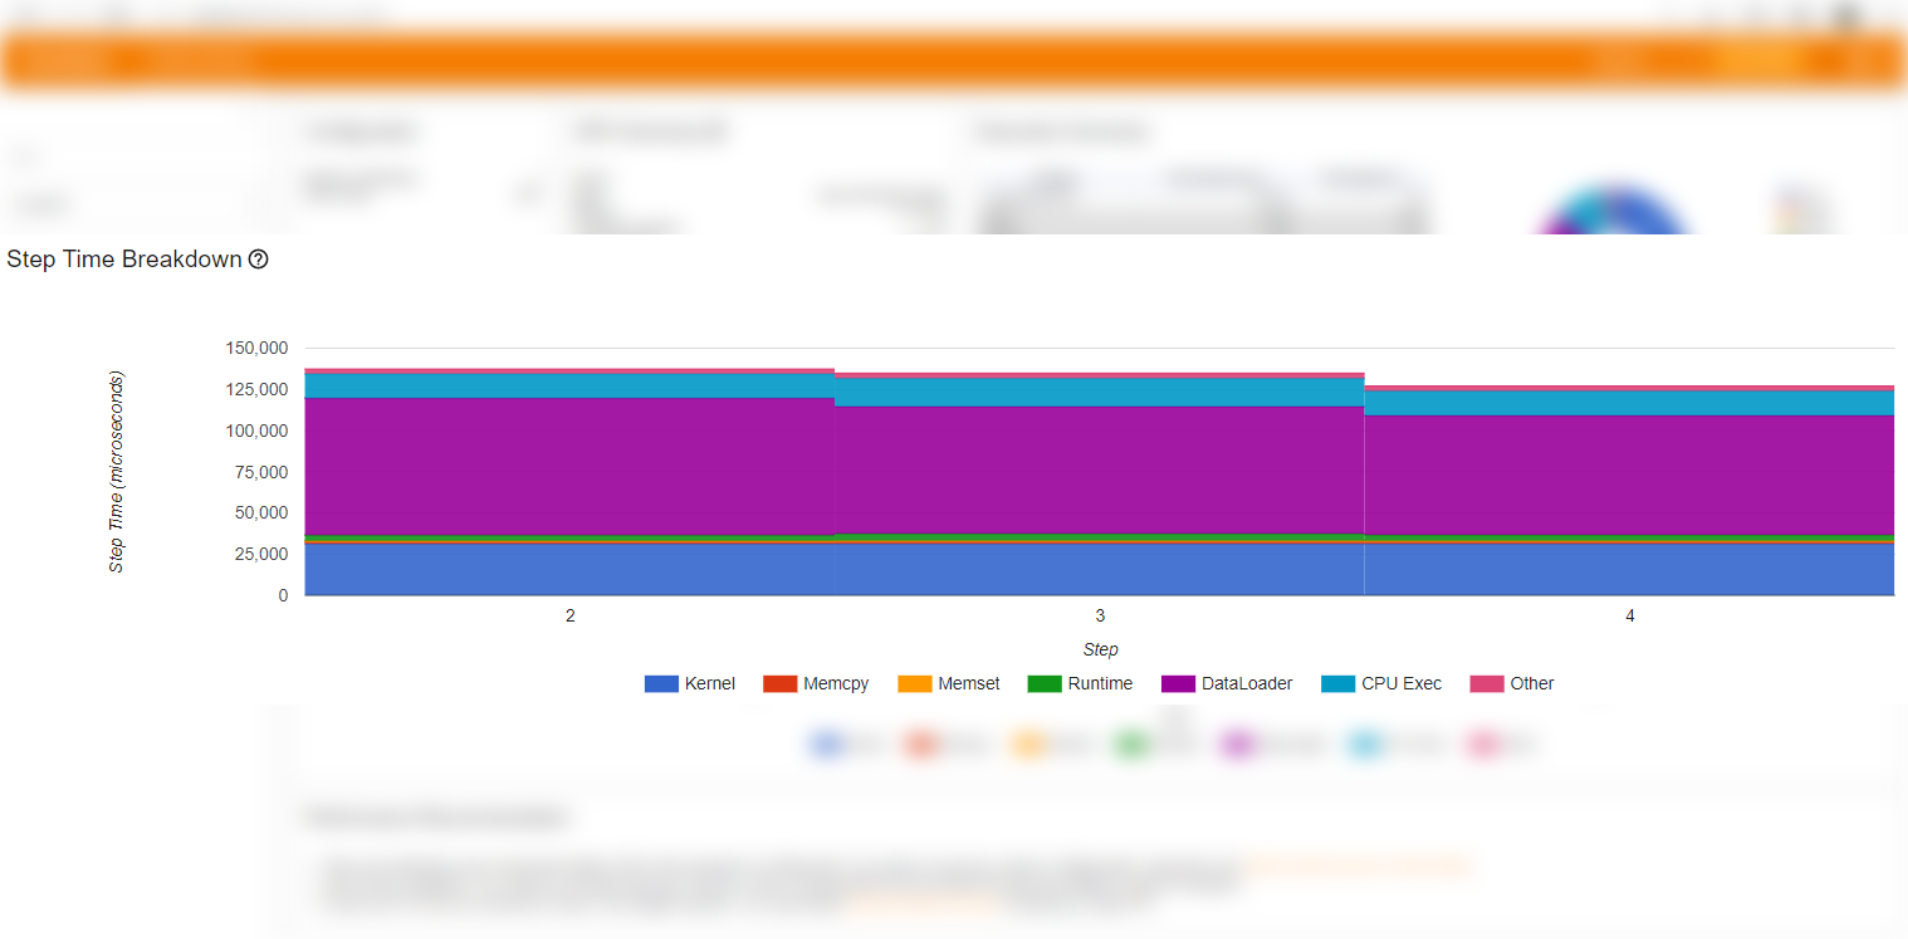
\includegraphics[width=1\textwidth]{assets/profiler_overview_step_time_breakdown}
    \end{figure}
    \end{center}
\source{Image source: Adapted from \url{https://pytorch.org/tutorials/intermediate/tensorboard_profiler_tutorial.html}, accessed on: 22.11.2022}

\end{frame}

\end{frame}

\begin{frame}{PyTorch Profiler With TensorBoard}
    \vspace{-1em}
    \begin{center}
    \begin{figure}
        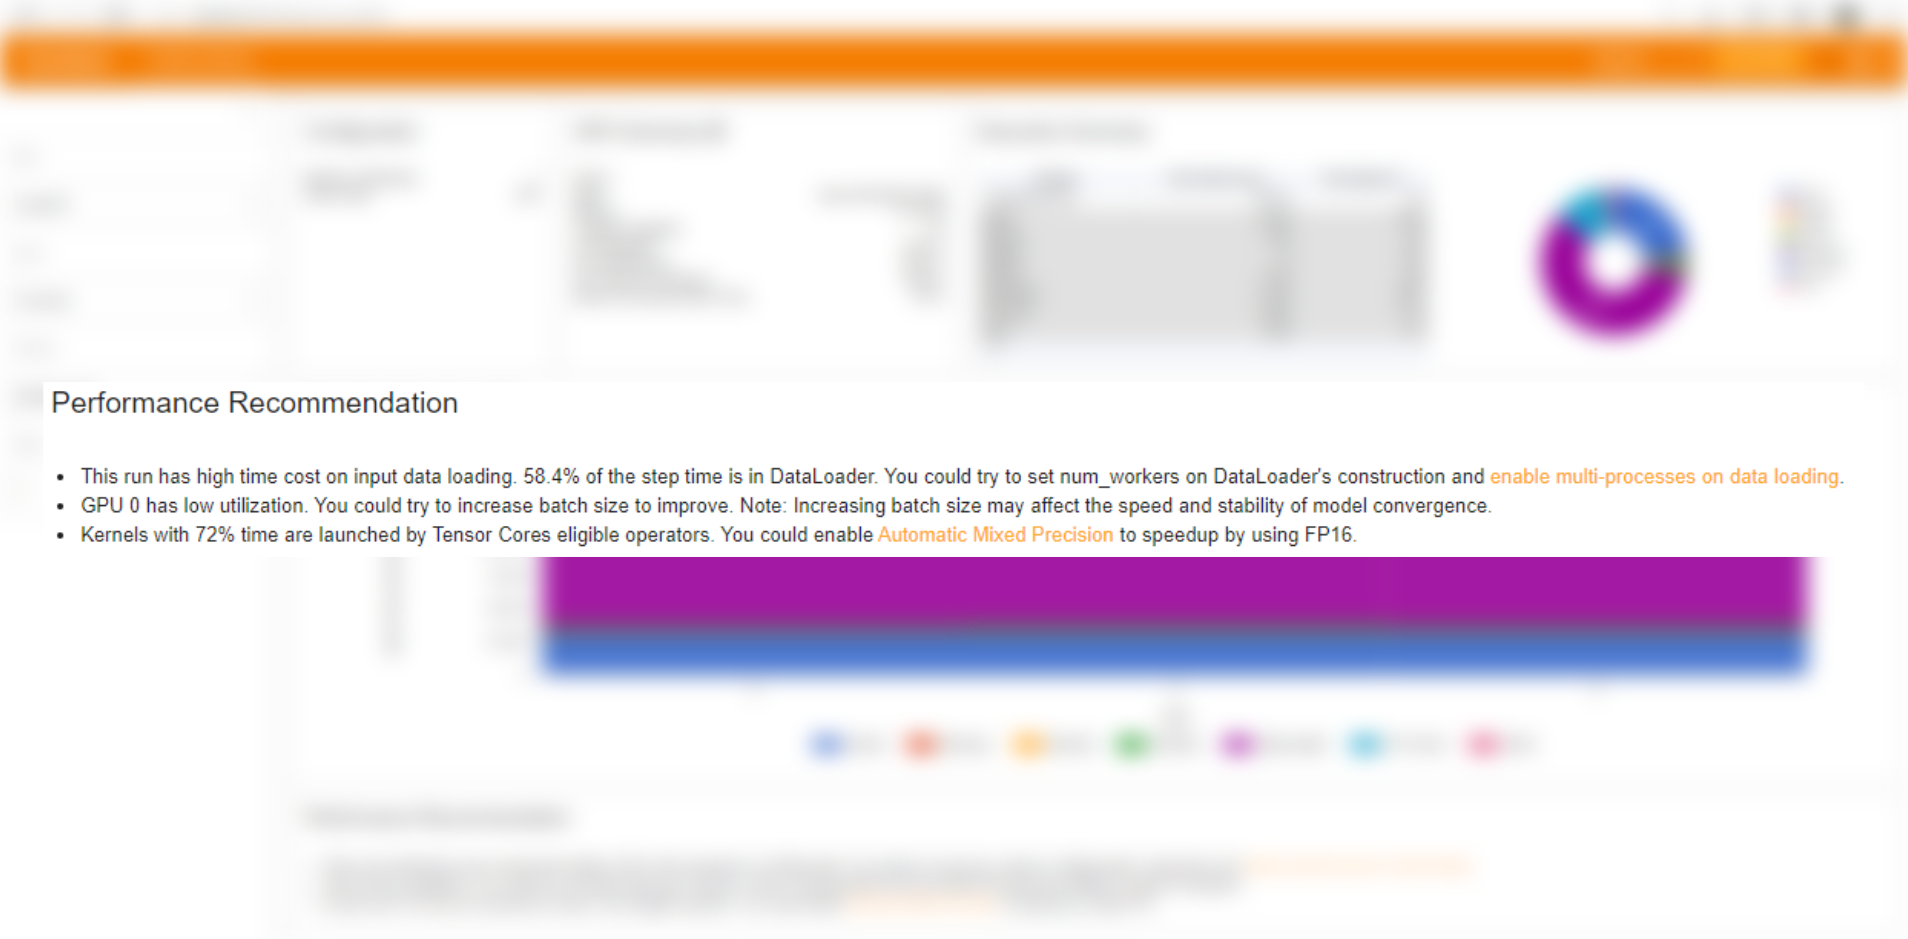
\includegraphics[width=1\textwidth]{assets/profiler_overview_performance_reccomondation}
    \end{figure}
    \end{center}
\source{Image source: Adapted from \url{https://pytorch.org/tutorials/intermediate/tensorboard_profiler_tutorial.html}, accessed on: 22.11.2022}

\end{frame}

\section{DeepSpeed - FlopsProfiler}
%\sectionIntroHidden % Show an outline of the current section with hidden subsections
\sectionIntro % Show an outline of the current section with subsections

\begin{frame}[fragile]{Summary}
    \vspace{-1em}
    \footnotesize\inputminted[xleftmargin=1em,linenos,fontsize=\scriptsize, firstline=1,lastline=20]{python}{./assets/deepspeed-flopsprofiler_example.txt }

\end{frame}

\begin{frame}[fragile]{Aggregated Profile per GPU}
    \vspace{-1em}
    \footnotesize\inputminted[xleftmargin=1em,linenos,fontsize=\scriptsize, firstline=28,lastline=46]{python}{./assets/deepspeed-flopsprofiler_example.txt }
    }

\end{frame}

\begin{frame}[fragile]{Detailed Profile per GPU}

    \footnotesize\inputminted[xleftmargin=1em,linenos,fontsize=\scriptsize, firstline=59,lastline=72, breaklines]{python}{./assets/deepspeed-flopsprofiler_example.txt }
    }

\end{frame}

\begin{frame}[fragile]{Torch profiler}
    \footnotesize\inputminted[xleftmargin=1em,linenos,fontsize=\scriptsize, highlightlines={4-10,14,15}]{python}{./assets/profiler-torch.py}

    \source{Tutorial: \url{https://pytorch.org/tutorials/intermediate/tensorboard_profiler_tutorial.html}, accessed on: 24.03.2023}
\end{frame}

\begin{frame}[fragile]{Deepspeed - FlopsProfiler}
    \vspace{-1em}
    \footnotesize\inputminted[xleftmargin=1em,linenos,fontsize=\scriptsize, highlightlines={1,3,4,8,9,11-18}]{python}{./assets/deepspeed.py}

    \source{Tutorial: \url{https://www.deepspeed.ai/tutorials/flops-profiler/}, accessed on: 24.03.2023}
\end{frame}

\section{Practical}

\begin{frame}{Profiling is the first step of optimizing}

\begin{columns}
        \begin{column}{0.5\textwidth}
            \centering
            \vspace{-1em}
            \begin{figure}
            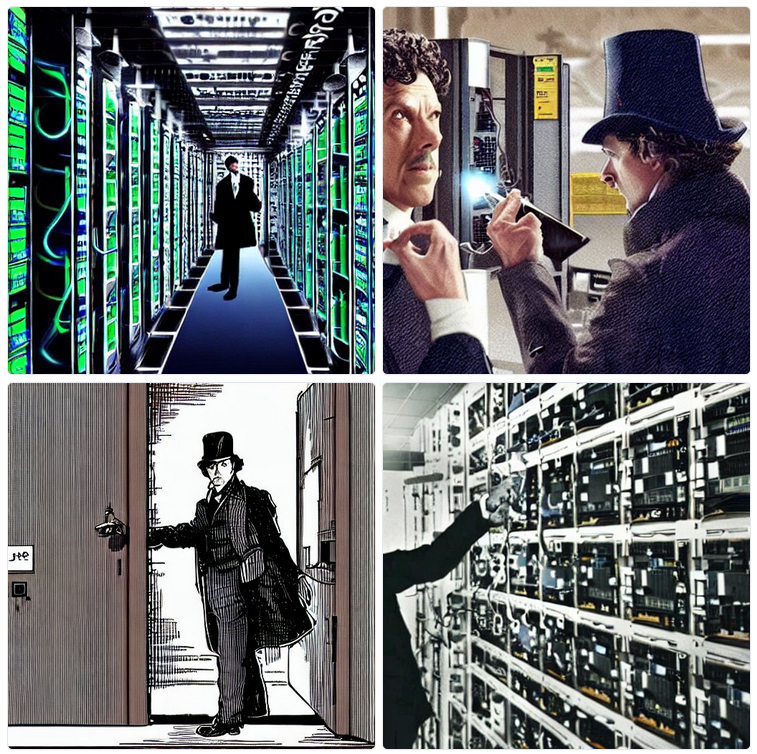
\includegraphics[width=0.85\textwidth]{assets/Sherlock-Holmes-locates-the-best-graphical-processing-unit-inside-the-data-center-for-his-deep-learning-workflow}
            \caption*{Image generated with stable diffusion: \\
            \tiny{"Sherlock Holmes locates the best graphical processing unit inside the data center for his deep learning workflow"}}
            \end{figure}
        \end{column}
        \begin{column}{0.5\textwidth}
            \begin{itemize}
                \item "Stable Diffusion v1 version of the model requires 150,000 A100 GPU Hours for a single training session"\footnote{\tiny{\url{https://syncedreview.com/2022/11/09/almost-7x-cheaper-colossal-ais-open-source-solution-accelerates-aigc-at-a-low-cost-diffusion-pretraining-and-hardware-fine-tuning-can-be/}}, accessed on: 10.11.2022}
                \vspace{1em}
                \item[$\Rightarrow$] Optimization of deep learning workflows is of growing importance for energy efficiency.
            \end{itemize}
        \end{column}
    \end{columns}

\end{frame}


\begin{frame}[fragile]{Practical}
\centering

\begin{block}{Task 1: Run the training job with the profilers. (15 min)}
    \begin{itemize}
        \item Add the code for using the profilers to \href{https://gitlab-ce.gwdg.de/dmuelle3/deep-learning-with-gpu-cores/-/blob/096a3d35e76d60ab557b150c9c3584a0f2c6e52c/code/train.py}{train.py}\footnote{a solution is provided in \href{https://gitlab-ce.gwdg.de/dmuelle3/deep-learning-with-gpu-cores/-/blob/096a3d35e76d60ab557b150c9c3584a0f2c6e52c/code/train_with_logger.py}{train_with_logger.py}}
        \item Set the number of epochs to 1 and interrupt the training after 5 batches of data (see \texttt{fast\_run} option in \texttt{train\_with\_logger.py})
        \item decrease time requested in SLURM to 20 minutes
        \begin{itemize}
            \item in \texttt{code/submit\_train.sh} $\rightarrow$ \texttt{\#SBATCH -t 00:20:00}
        \end{itemize}
    \end{itemize}
\end{block}

\end{frame}

\begin{frame}[fragile]{Practical}
\label{pg:lastpage} % Label on last frame to get the page number for footer
\centering
\begin{block}{Task 2: Analyze the profilers output (15 min)}
\begin{itemize}
    \item Download the output of the PyTorch profiler and visualize it with TensorBoard
    \item The output of DeepSpeed's FlopsProfiler is in the slurm output file
    \item An example output of the profilers can be found in our course directory
    \begin{itemize}
        \item Instructions on how to use them can be found in the \href{https://gitlab-ce.gwdg.de/dmuelle3/deep-learning-with-gpu-cores/-/tree/main/#download-and-visualize-profiling-results-of-example-run}{README}
    \end{itemize}
\end{itemize}
\end{block}
\end{frame}

\begin{frame}{References}
    % References slide in appendix
    \renewcommand*{\bibfont}{\normalfont\scriptsize}
    \printbibliography[heading=none]
\end{frame}

\begin{frame}{Course Agenda}
\centering
\includegraphics[width=0.9\textwidth]{assets/dlgpu_agenda}
\end{frame}

\end{document}
